\chapter{Analyse}
\label{cha:Analyse}


\section{Anforderungsanalyse}
Für die Anforderungsanalyse wurde aufgrund der Projekt- und Applikationsgrösse das User-Stories Verfahren gewählt. Für die Ausarbeitung der Anforderungen wurde ein kleines Gremium zusammengestellt, welche die einzelnen Interessengruppen vertreten. Zu den Intressengruppen gehören der Teamleiter, die Storage Admins, die Capacity Planer und der System Admin und System Engineer. 
Die Use Cases wurden anschliessend in zwingende Anforderungen und nicht-zwingende Anforderungen unterteilt.

\textbf{Lukas (System Engineer):}

\fbox{\parbox{\linewidth}{Mit dem Tool vorgenommene Änderungen müssen aufgezeichnet (geloggt) werden.}}

\fbox{\parbox{\linewidth}{Bevor die Änderungen vorgenommen werden, soll eine Zusammenfassung angezeigt werden (idealierweise mit graphischer Darstellung)}}\newline\newline

 
\textbf{Thorsten (Storage Admin):}

\fbox{\parbox{\linewidth}{Als Storage Admin kann ich den Storage End-to-End bis zum Filesystem bereitstellen}}

\fbox{\parbox{\linewidth}{Als Capacity Planer kann ich mir schnell und einfach einen Überblick über den benutzten und verfügbaren Diskspace verschaffen}}

\fbox{\parbox{\linewidth}{Als User kann ich einfach neuen Diskspace auf meinem Server bestellen und kann den Workflow verfolgen.}}\newline\newline


\textbf{Daniel (System Admin):}

\fbox{\parbox{\linewidth}{Als System Admin kann ich das Volumes des Servers vergrössern, ohne LVM Befehle kennen zu müssen}}

\fbox{\parbox{\linewidth}{Als System Admin kann ich beim Vergrössern der Volumes automatisch das Filesystem vergrössern}}

\fbox{\parbox{\linewidth}{Als System Admin kann ich ein Site-übergreifendes Mirroring einrichten}}

\fbox{\parbox{\linewidth}{Als System Admin kann ich den Diskspace auf ein anderes Storage System migrieren }}

\fbox{\parbox{\linewidth}{Als System Admin werde ich beim sicheren Entfernen eines Disk eines gewählten Servers von der Anwendung unterstützt }}

\fbox{\parbox{\linewidth}{Als System Admin erhalte ich einen raschen Überblick über die Diskkonfiguration des zu wartenden Servers}}\newline\newline

\textbf{David (Teamleiter):}

\fbox{\parbox{\linewidth}{Als Teamleiter kann ich nachvollziehen wer, wann welche Änderung vorgenommen hat}}

\fbox{\parbox{\linewidth}{Als Applikation Owner kann ich den zugewiesenen Diskplatz prüfen}}

\textbf{Philipp (Capacity Admin):}

\fbox{\parbox{\linewidth}{Als Capacity Planer kann ich eine Storagereservation vornehmen }}

\fbox{\parbox{\linewidth}{Als Capacity Planer erhalte ich einen raschen Überblick auf die noch unbenutzten Storages }}


\subsection{Zwingend}

Die folgenden Anforderungen müssen zwingend umgesetzt werden:

\begin{itemize}
\item Als System Admin kann ich das Filesystem des Server vergrössern, ohne LVM Befehle zu kennen
\item Als System Admin kann ich Storage am Server wieder reduzieren
\item Als System Admin erhalte ich einen raschen Überblick über die Diskkonfiguration des Servers
\item Als User kann ich einfach neuen Diskspace auf meinem Server bestellen und kann den Workflow verfolgen.
\item Die dem vom Tool vorgenommenen Änderungen müssen aufgezeichnet (geloggt) werden.
\end{itemize}

\subsection{Nicht zwingend}

Die folgenden Anforderungen, werden in diesem Projekt nicht umgesetzt, auch wenn einige davon für eine Produktiveversion interessante und wichtige Anforderungen wären:

\begin{itemize}
\item Als Capacity Planer kann ich Storage reservieren
\item Als Applikation Owner kann ich den zugewiesenen Diskplatz prüfen
\item Als Capacity Planer kann ich mir schnell und einfach einen Überblick über den benutzten und verfügbaren Diskspace verschaffen
\item Bevor die Änderungen vorgenommen werden, soll eine Zusammenfassung (idealerweise graphisch dargestellt) angezeigt werden
\end{itemize}


\section{Marktanalyse}
\subsection{Potenzielle Kunden}
Unternehmen konkurrenzieren sich nicht nur im Produkteverkauf und bei der Aquisition von neuen Kunden, sonder auch bei der effizienten Gestaltung der internen Abläufe und optimalen Nutzung der eigenen Ressourcen. Seit Beginn des Computerzeitalters hat die Bedeutung der IT in ausnahmslos allen Unternehmen stark zugenommen. Unternehmen mit einer schlecht funktionierenden IT-Infrastruktur verlieren am Markt an Konkurrenzstärke und manövrieren sich über kurz oder lang auf das Abstellgeleise mit einer unsicheren Zukunft. Eine moderne Geschäftsleitung hat dies längst erkannt und legt Wert auf die Erhaltung und den Ausbau der inneren Stärke in Bezug auf die Abstimmung der Business-Strategie mit der Leistung der IT. Was nützt der beste Verkäufer, wenn es nach dem Verkaufsabschluss mit der Umsetzung des Auftrages happert.

Die Autoren \Autor{4755749} haben in einem Artikel über das Thema IEEE, die Frage der CIO-Charakteristik zur Unternehmensstrategie untersucht:

\begin{quote}
"''In a diverse, ever-changing marketplace, organizations are constantly seeking to harness technology to improve their core competency and gain competitive advantage. \textbf{Explicitly, knowing how to apply Information Systems (IS) in an appropriate and timely way and in harmony with business strategies, goals, and needs could bring the organization to steps closer to business success.} In other words, aligning IS strategy to business strategy becomes a critical issue in most organizations. Indeed, there is an increasing amount of research and understanding on the linkages between business and IS strategies, the role of partnerships between IS and business management, and the need to understand the transformation of business strategies resulting from the competitive use of IS."'' \footnote{\Zitat[S.~1]{4755749}}
\end{quote}


Trotz der zunehmenden Bedeutung der IT-Leistung für die innerbetrieblichen Abläufe aber auch vermehrt direkt an der Verkaufsfront, steigt der Druck an stetiger Optimierung und effizienteren Verarbeitung der IT-Prozesse in den IT-Abteilungen. Zusätzlicher Druck von Aussen bezüglich politischen und marktwirtschaftlichen Veränderungen, ich denke da zB. an neue Gesetze und Regulatorien, erhöht die Erwartungen an die IT Dienstleistung.
Unternehmen vergleichen sich heute immer mehr an der Leistungsfähigkeit ihrer IT-Leistung wie zB. bezüglich der Kostenstruktur oder Funktionalität mit der Konkurrenz. Schneidet die Effizienz der IT-Abteilung (Leistung versus Kosten) schlecht ab, sind die Gegenmassnahmen oft drastisch und erfordert höchste Konzentration des IT-Managements. Zu nennen sind da unter anderem massive Kosteneinsparungen, Streichung oder Aufschiebung von Projekten, Entlassung von internen und externen Mitarbeiter, Outsourcing bzw. Insourcing, um nur einige der möglichen Massnahmen aufzuführen. Dass solche Eingriffe  den IT-Betrieb zusätzlich lähmen kann versteht sich von selbst. Eine laufende Überprüfung und Verbesserung der eigenen Organisation und Kostenstruktur gehört zum Tagesgeschäft des erfolgreichen IT-Managers. Es verwundert nicht, dass daraus auch neue Modell entstehen, wie zB. das anbieten der IT-Dienstleistung als Profit-Center innerhalb des Gesamtbetriebes, die Auslagerung der Dienste ins Ausland nach dem Outsourcing Modell der Inder oder die Aufsplittung der Services in Production und Engineering. In diesem Sinn ist dieses Projekt zu verstehen, indem eben die Storage-Verwaltung vereinfacht und effizienter gestaltet werden soll, um damit einen vielleicht kleinen, aber wichtigen Beitrag zur Verringerung der IT-Kosten zu erfüllen. 


\subsection{Server Markt}
\subsubsection{Betriebsystem}
Waren vor ein paar Jahren Linux-Installationen im Server-Bereich, meist als ideologisch und experimentell angesehen, hat sich dies in der Zwischenzeit gewandelt.
Vermehrt wird Linux für Hosting- und Web-Installationen in Klein- bis Grossbetrieben professionell eingesetzt und hat Boden gegenüber von dominierenden Windows-Server-Installationen gutgemacht. Dank zunehmender Unterstützung seitens Software Herstellern für die Linux-Plattform steigt das Interesse an Linux im professionellen Geschäftsumfeld. Vergleicht man das Angebot der Betriebsystem Hersteller Oracle, IBM und Microsoft mit dem Angebot der beiden Linux Distributoren Red Hat und Novell Suse, ist ersichtlich, dass sich die Angebote bezüglich Wartung, Support und Dienstleistungen nicht wesentlich voneinander unterscheiden. 
Trotz diesem heute breiten Angebot an Funktionalität im Linux Umfeld, konnte sich dieses Betriebsystem bis anhin im Finanzdienstleistungs-Branche bei den Unternehmen nicht durchsetzen, ausser für dedizierte Web-Installationen. Traditionell dominieren in diesem Marktsegment immer noch die Betriebsysteme wie Windows, Oracle Solaris (SUN) bzw. IBM AIX als die strategisch geführten Plattformen. Es gibt jedoch Anzeichen, dass sich dieses Verhältnis künftig ändern könnte, denn einige Unternehmen haben für neue Projekte ein Auge auf Linux neben Windows geworfen und liebäugeln Linux nun auch als strategische  Betriebsystem Plattform einzusetzen.

\subsubsection{Hardware Platform}
\begin{figure}[htb]
\centering
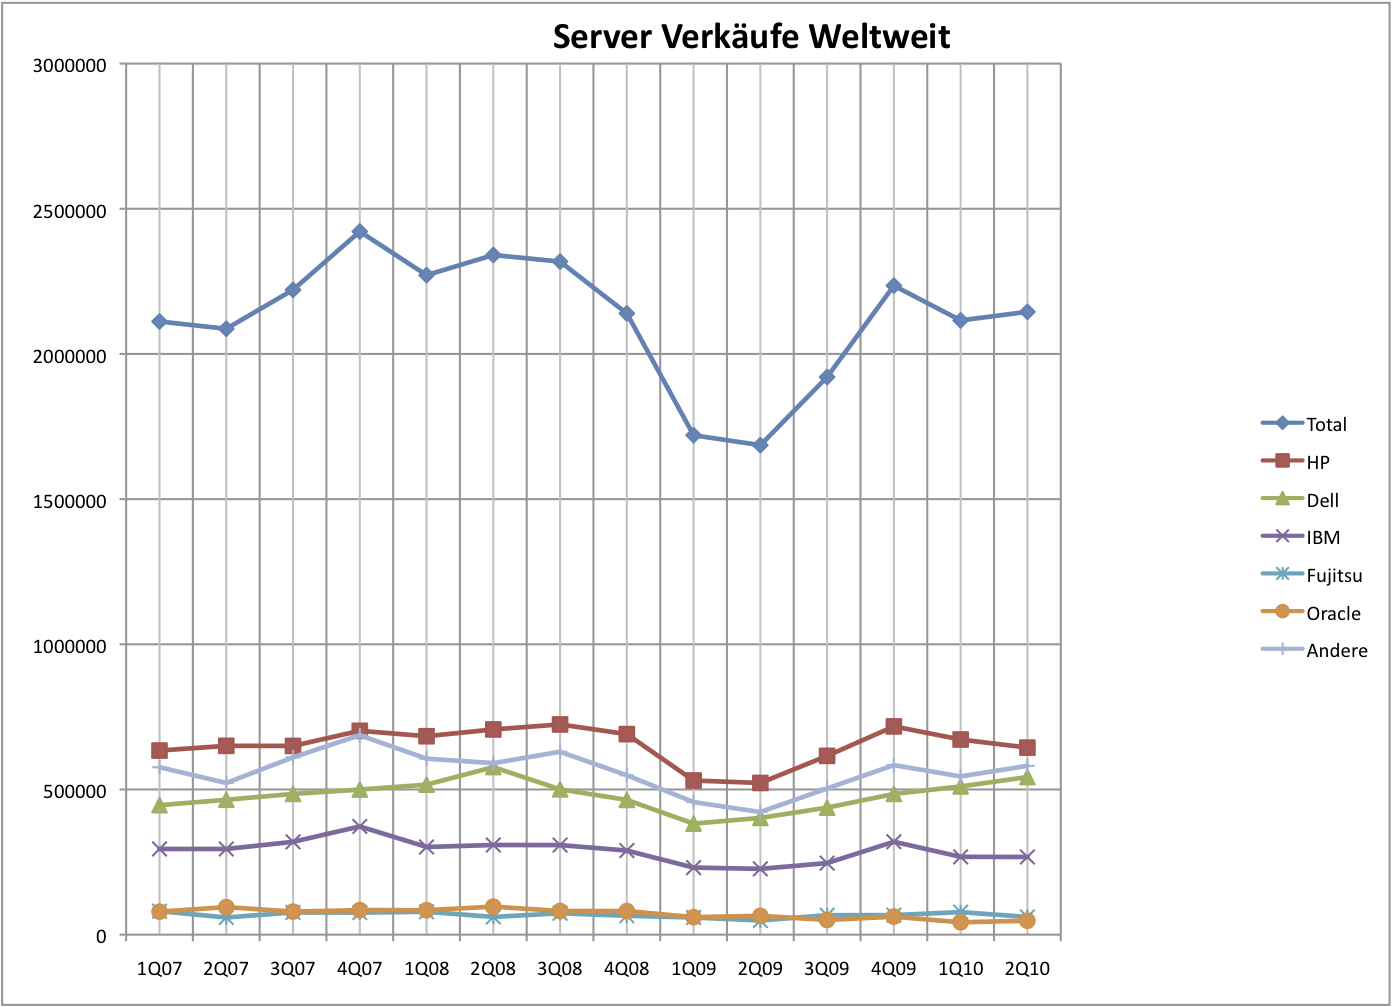
\includegraphics[width=1\textwidth]{DiagrammServerVerkaufeWeltweitQuartal.png}
\caption{Diagramm - Server Verkauf: Weltweit pro Quartal \textit{Quelle Gartner}}
\label{fig:DiagrammServerVerkaufeWeltweitQuartal}
\end{figure}

Ein möglicher Faktor für die zunehmende Ablösung der Betriebsysteme Solaris und AIX durch Linux könnte deren Hardware Plattform, welche zumeist auf RISC bzw. Intanium Prozessoren basieren, sein. 
Im Low- und Midrange Bereich sind solche Hardware Systeme nicht gleich Leistungsfähig wie Systeme welche auf den x86 bzw. die x64 Prozessor-Architektur aufgebaut sind. Zudem lassen die höheren Kosten für den Betrieb und Unterhalt von zwei unterschiedlichen Hardware-Plattformen innerhalb deselben Unternehmens solche Projekte verständlicherweise in den Hintergrund drängen.
Diese Einschätzung decken sich auch mit der Server-Hardware Marktanteil Analyse vom zweiten Quartal 2010 von Gartner. Die x86 basierenden Systeme sind um 28.9 Prozent in der verkauften Stückzahl und in 37 Prozent im Umsatz gewachsen. RISC/Itanium basierenden Systeme haben im gleichen Zeitraum  im Vergleich zum selben Vorjahresquartal 16.5 Prozent bezüglich der verkauften Stückzahlen sowie 8.8 Prozent beim Umsatz verloren.

Das Linien-Diagramm der \abbildung{DiagrammServerVerkaufeWeltweitQuartal} zeigt die Anzahl verkauften Servern der einzelnen Herstellern vom ersten Quartal 2007 bis zum zweiten Quartal 2010. 
Aus dem Diagramm kann man nicht direkt erkennen, dass die x86/x64 Prozessor-Architektur bei den Servern im Vergleich zu RISC bzw. Itanium Prozessoren überwiegt. Neben HP und Dell, welche hauptsächlich x86/X64 Server verkaufen, ist Oracle einer der führenden RISC Server Hersteller bezüglich der Anzahl verkaufter Server weit abgeschlagen. Zudem kann man aus den \tabelle{WeltServerWarenlieferung2010} und \tabelle{EMEAServerWarenlieferung2010} erkennen, dass Oracle im zweiten Quartal 2010 gegenüber der Konkurrenz den stärksten Abastzrückgang erleiden musste.

Gemäss Herrn O'Connell von Garnter sind die Rückgänge vom RISC/Itanium Segment auf die folgenden Ursachen rückzuführen:

\begin{quote}
“'The first half of 2010 has seen continued challenges for vendors in the server segment of RISC and Itanium Unix. The combination of longer sales cycles for these systems, product refreshes and ongoing economic uncertainty has resulted in RISC/Itanium Unix revenue in the second quarter of 2010 being less than half that of the second quarter of 2008, we expect this market to improve in the second half of 2010, but vendors in this segment will face an increasingly difficult challenge in minimizing migrations to Windows and Linux platforms.”'
\footnote{O’Connell, http://www.gartner.com/it/page.jsp?id=1426834}
\end{quote}

Wie man in der Tabelle \ref{tab:WeltServerWarenlieferung2010} von Gartner über die weltweiten Server Warenlieferungen im zweiten Quartal 2010 erkennen kann, haben die beiden grössten Server Hersteller mit RISC Architektur eine Wachstumsverlangsamung gegenüber dem gleichen Quartal 2009 in Kauf nehmen müssen. Die restlichen Hersteller hatten ein der selben Periode ein positives Wachstum verzeichnet. Bei IBM ist diese Zahl wenig aussagefähig, da nicht hervorgeht wie der Rückgang der Zahlen auf die Produkte bezüglich Prozessor Architektur aufzuteilen sind.


\begin{longtable}{|m{1,7cm}|m{2,3cm}|m{1,4cm}|m{2,2cm}|m{1,4cm}|m{1,3cm}m{0.01mm}|}
\caption{ Weltweite: Hersteller Server Warenlieferung Q2 2010 (Stück)} \\
\hline
\label{tab:WeltServerWarenlieferung2010}
& Q2 10 &  Q2 10 & Q2 09 & Q2 09 & Q2 09 - Q2 10 & \\
\textbf{Hersteller}& \textbf{Stückzahl}& \textbf{Markt- Anteil}& \textbf{Stückzahl}& \textbf{Markt- Anteil} &\textbf{Wach- stum}&\\
\hline
HP & \raggedleft 644'172 &\raggedleft  30,0 \% & \raggedleft 522'447 & \raggedleft 31,0 \% &  \raggedleft 23,3 \% & \\
\hline
Dell & \raggedleft 542'799 & \raggedleft 25,3 \% & \raggedleft 402'187 & \raggedleft 23,8 \% &\raggedleft 35,0 \%& \\
\hline
IBM & \raggedleft 267'614 & \raggedleft 12,5 \% & \raggedleft 226'570 & \raggedleft 13,4 \% & \raggedleft 18,1 \% &\\
\hline
Fujitsu &\raggedleft 60'974 &\raggedleft 2,8 \%  & \raggedleft 48'819 & \raggedleft 2,9 \% &  \raggedleft 24,9 \% &\\
\hline
Sun & \raggedleft 47'968 & \raggedleft 2,2 \%  & \raggedleft 64'810 & \raggedleft 3,8 \% & \raggedleft  -26,0 \% &\\
\hline
Andere Hersteller & \raggedleft 581'512 & \raggedleft 27,1 \%  & \raggedleft 422'371 & \raggedleft 37,7 \% &  \raggedleft 27,1 \%& \\
\hline
\hline
\textbf{Total} & \raggedleft 2'145'039 & \raggedleft 100,0 \%  &\raggedleft 1'687'204 & \raggedleft 100,0 \% &  \raggedleft 27,1 \% &\\
\hline
\end{longtable}


\begin{longtable}{|m{1,7cm}|m{2,3cm}|m{1,4cm}|m{2,2cm}|m{1,4cm}|m{1,3cm}m{0.01mm}|}
\caption{ Weltweite: Hersteller Server Warenlieferung Q2 2009 (Stück)} \\
\hline
\label{tab:WeltServerWarenlieferung2009}
& Q2 09 &  Q2 09 & Q2 08 & Q2 08 & Q2 08 - Q2 09 & \\
\textbf{Hersteller}& \textbf{Stückzahl}& \textbf{Markt- Anteil}& \textbf{Stückzahl}& \textbf{Markt- Anteil} &\textbf{Wach- stum}&\\
\hline
HP & \raggedleft 522'447 &\raggedleft  31,0 \% & \raggedleft 706'724 & \raggedleft 30,2 \% &  \raggedleft -26,1 \% & \\
\hline
Dell & \raggedleft 402'187 & \raggedleft 23,9 \% & \raggedleft 577'163 & \raggedleft 24,7 \% &\raggedleft -30,3 \%& \\
\hline
IBM & \raggedleft 226'570 & \raggedleft 13,4 \% & \raggedleft 308'835 & \raggedleft 13,2 \% & \raggedleft -26,6 \% &\\
\hline
Sun &\raggedleft 63'412 &\raggedleft 3,8 \%  & \raggedleft 96'510 & \raggedleft 4,1 \% &  \raggedleft -26,6 \% &\\
\hline
Fujitsu & \raggedleft 48'819 & \raggedleft 2,9 \%  & \raggedleft 61'077 & \raggedleft 2,6 \% & \raggedleft  -20,1 \% &\\
\hline
Andere Hersteller & \raggedleft 422'371 & \raggedleft 25,1 \%  & \raggedleft 590'468 & \raggedleft 25,2 \% &  \raggedleft -28,5 \%& \\
\hline
\hline
\textbf{Total} & \raggedleft 1'685'806 & \raggedleft 100,0 \%  &\raggedleft 1'687'204 & \raggedleft 100,0 \% &  \raggedleft -28,0 \% &\\
\hline
\end{longtable}


\begin{longtable}{|m{1,7cm}|m{2,3cm}|m{1,4cm}|m{2,2cm}|m{1,4cm}|m{1,3cm}m{0.01mm}|}
\caption{ EMEA: Server Hersteller Warenlieferung Q2 2010 (Stück)} \\
\hline
\label{tab:EMEAServerWarenlieferung2010}
& Q2 10 &  Q2 10 & Q2 09 & Q2 09 & Q2 09 - Q2 10 & \\
\textbf{Hersteller}& \textbf{Stückzahl}& \textbf{Markt- Anteil}& \textbf{Stückzahl}& \textbf{Markt- Anteil} &\textbf{Wach- stum}&\\
\hline
HP & \raggedleft 241'898 &\raggedleft  41,5 \% & \raggedleft 200'421 & \raggedleft 40,6 \% &  \raggedleft 20,7 \% & \\
\hline
Dell & \raggedleft 111'328 & \raggedleft 19,1 \% & \raggedleft 90'273 & \raggedleft 18,3 \% &\raggedleft 23,3 \%& \\
\hline
IBM & \raggedleft 63'701 & \raggedleft 10,9 \% & \raggedleft 62'359 & \raggedleft 12,6 \% & \raggedleft 2,2 \% &\\
\hline
Fujitsu &\raggedleft 36'575 &\raggedleft 6,3 \%  & \raggedleft 31'207 & \raggedleft 6,3 \% &  \raggedleft 17,2 \% &\\
\hline
Sun & \raggedleft 15'473 & \raggedleft 2,7 \%  & \raggedleft 24'053 & \raggedleft 4,9 \% & \raggedleft  -35,7 \% &\\
\hline
Andere Hersteller & \raggedleft 114'558 & \raggedleft 19,6 \%  & \raggedleft 84'743 & \raggedleft 17,2 \% &  \raggedleft 35,2 \%& \\
\hline
\hline
\textbf{Total} & \raggedleft 583'533 & \raggedleft 100,0 \%  &\raggedleft 492'056 & \raggedleft 100,0 \% &  \raggedleft 18,4 \% &\\
\hline
\end{longtable}

\begin{longtable}{|m{1,7cm}|m{2,3cm}|m{1,4cm}|m{2,2cm}|m{1,4cm}|m{1,3cm}m{0.01mm}|}
\caption{ EMEA: Hersteller Server Warenlieferung Q2 2009 (Stück)} \\
\hline
\label{tab:EMEA:ServerWarenlieferung2009}
& Q2 09 &  Q2 09 & Q2 08 & Q2 08 & Q2 08 - Q2 09 & \\
\textbf{Hersteller}& \textbf{Stückzahl}& \textbf{Markt- Anteil}& \textbf{Stückzahl}& \textbf{Markt- Anteil} &\textbf{Wach- stum}&\\
\hline
HP & \raggedleft 200'421 &\raggedleft  40,8 \% & \raggedleft 293'621 & \raggedleft 40,6 \% &  \raggedleft -31,7 \% & \\
\hline
Dell & \raggedleft 90'273 & \raggedleft 18,4 \% & \raggedleft 138'000 & \raggedleft 19,1 \% &\raggedleft -34,6 \%& \\
\hline
IBM & \raggedleft 62'359 & \raggedleft 12,7 \% & \raggedleft 95'861 & \raggedleft 13,3 \% & \raggedleft -34,9 \% &\\
\hline
Fujitsu &\raggedleft 31'207 &\raggedleft 6,3 \%  & \raggedleft 40'775 & \raggedleft 5,6 \% &  \raggedleft -23,5 \% &\\
\hline
Sun & \raggedleft 22'655 & \raggedleft 4,6 \%  & \raggedleft 30'584 & \raggedleft 4,2 \% & \raggedleft  -25,9 \% &\\
\hline
Andere Hersteller & \raggedleft 84'743 & \raggedleft 17,2 \%  & \raggedleft 123'561 & \raggedleft 17,1 \% &  \raggedleft -31,4 \%& \\
\hline
\hline
\textbf{Total} & \raggedleft 491'658 & \raggedleft 100,0 \%  &\raggedleft 722'402 & \raggedleft 100,0 \% &  \raggedleft -31.9 \% &\\
\hline
\end{longtable}

Der Betriebsystemhersteller Microsoft hat angekündigt, nach Windows 2008 R2 keine Software mehr für Itanium Prozessoren zu entwickeln. Ferner verzichten auf den Support von Itanium in ihren zukünftigen Softwareversionen die beiden Linux Distrbutoren RedHat (RedHat Enterprise Linux) und Canonical (Ubuntu Linux). Canonical wird zusätzlich den Sparc Support einstellen. Diese Hersteller sind zwar bei den Installationen auf den genannten Prozessoren eher Nischenanbieter, jedoch unterstützt dies die These, dass die Hersteller künftig ihre Produktstrategie nicht mehr auf diese Prozessoren richten.


\subsubsection{Konkurrenzprodukt}
Der internationale Softwarekonzern Symantec Corporation mit Hauptsitz in Cupertino Kalifornien, hat mit der Veritas Storage Foundation Suite ein umfangreiches Portfolio für Volume Manager, File System und Storage Manager im Angebot. Mit dem Produkt Veritas Storage Foundation Manager hat Symantec eine vergleichbare Lösung wie die geplante Volume Managment Engine. Mit dem Veritas Storage Foundation Manager lässt sich zentral über ein Web-GUI die Server Volumes verwalten. 
Der Veritas Storage Foundation Manager unterstützt jedoch nur ihren eigenen Volume Manager. Deshalb kann der Betriebsystem eigene Volume Manager nicht verwendet werden. Folgende Betriebsysteme werden unterstützt: Oracle Solaris, HP HP-UX, IBM AIX, Linux und Microsoft Windows.

RedHat bietet mit der Opensource Applikation Conga, eine webbasierende Linux Cluster und LVM Verwaltungslösung an. Die Applikation ist jedoch auf das Verwalten der Konfiguration beschränkt.